\documentclass{../../slides-style}

\slidetitle{Сложность алгоритмов}{13.09.2023}

\begin{document}
    
    \begin{frame}[plain]
        \titlepage
    \end{frame}
    
    \begin{frame}
        \frametitle{Сложность}
        \begin{itemize}
            \item Быстрее --- не значит лучше!
            \begin{itemize}
                \item Время работы программиста может быть дороже времени работы программы
                \item Но может быть и наоборот, если программа часто используется
            \end{itemize}
            \item Сложность
            \begin{itemize}
                \item Вычислительная (время работы)
                \item Емкостная (объём потребляемой памяти)
                \item Они взаимосвязаны
            \end{itemize}
            \item Вычислительную сложность непонятно, как измерять
            \begin{itemize}
                \item Зависит от машины, на которой считаем
                \item Зависит от объёма входных данных
                \item Зависит от самих входных данных
            \end{itemize}
        \end{itemize}
    \end{frame}

    \begin{frame}
        \frametitle{Асимптотическая сложность}
        \begin{itemize}
            \item O-символика
            $$f(n) \in O(g(n))$$
            $$\exists C > 0, n_0 : \forall n > n_0\;\; f(n) \leq C(g(n))$$
            \item То есть ``$f$ принадлежит классу функций $O(g)$, если начиная с некоторого $n_0$ она ограничена сверху функцией $g$ с точностью до некоторого наперёд заданного множителя''
            \item Или ещё более то есть --- ``f растёт не быстрее g''
        \end{itemize}
    \end{frame}

    \begin{frame}
        \frametitle{Пример}
        \begin{center}
            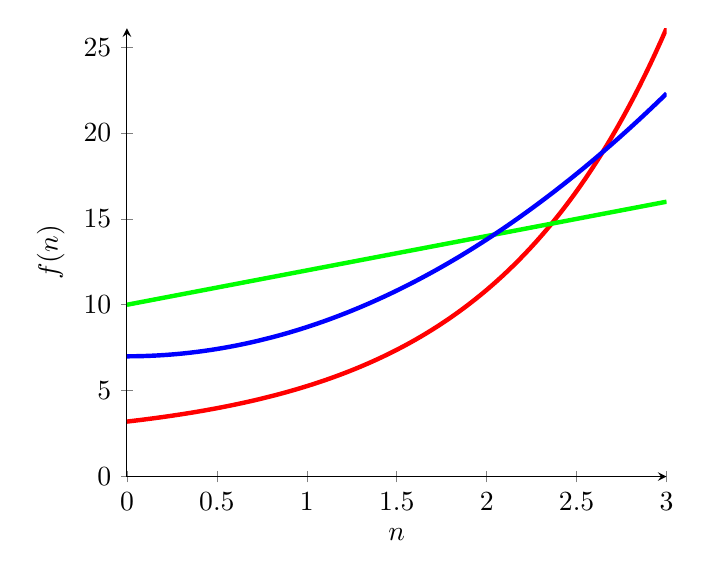
\begin{tikzpicture}
                \begin{axis}[
                        axis lines = left,
                        xlabel = $n$,
                        ylabel = {$f(n)$},
                        ymin = 0,
                        every axis plot/.append style={ultra thick}
                    ]
                    \addplot [
                            domain=0:3, 
                            samples=100, 
                            color=red,
                        ]
                    {1.2*exp(x) + 2};
                    \addplot [
                            domain=0:3, 
                            samples=100, 
                            color=green,
                        ]
                    {2*x + 10};
                    \addplot [
                            domain=0:3, 
                            samples=100, 
                            color=blue,
                        ]
                    {1.7*x^2 + 7};
                \end{axis}
            \end{tikzpicture}
        \end{center}
    \end{frame}

    \begin{frame}
        \frametitle{Правила вычисления трудоёмкости}
        \begin{itemize}
            \item Оператор $S_1$ выполняется за время $T_1(n)$, имеющее порядок $O(f(n))$, оператор $S_2$ --- за время $T_2(n)$, имеющее порядок $O(g(n))$, тогда $S_1$; $S_2$ выполняется за время $O(max(f(n), g(n)))$
            \begin{itemize}
                \item Следствие: $O(n^2 + n)$ = $O(n^2)$
            \end{itemize}
            \item Если $S_1$ внутри себя порядка $O(f(n))$ раз вызывает $S_2$, то итоговая трудоёмкость равна $O(f(n) * g(n))$
            \begin{itemize}
                \item Это правило позволяет анализировать циклы
            \end{itemize}
        \end{itemize}
    \end{frame}
    
        \begin{frame}[fragile]
        \frametitle{Пример: пузырёк}
        \begin{footnotesize}
            \begin{minted}{cpp}
for (int i = 0; i < n; ++i)                  // O((n - 1) + … + 1) = O(n * (n - 1) / 2) = O(n^2)
    for (int j = n; j > i; --j)                 // O((n - i) * 1) = O(n - i)
        if (a[j - 1] > a[j])                      // O(1)
             swap(a[j - 1], a[j]);            // O(1)
            \end{minted}
        \end{footnotesize}

        \begin{itemize}
            \item Бывают сортировки за $O(n*log(n))$
            \item Бывает сортировка подсчётом, за $O(n)$
            \item Это важно, $log_2(1000000) \sim 20$
            \begin{itemize}
                \item Обратите внимание, $O(log_2(n)) = O(ln(n))$
            \end{itemize}
        \end{itemize}
    \end{frame}

    \begin{frame}[fragile]
        \frametitle{Анализ рекурсивных алгоритмов}
        \begin{footnotesize}
            \begin{minted}{cpp}
int recursiveFactorial(int a) {
      if (a <= 1)
              return 1;
      else
              return a * recursiveFactorial(a - 1);
}
            \end{minted}
        \end{footnotesize}
        \begin{itemize}
            \item $T(n) = c + T(n-1)$ при $n > 1$, и $d$, при $n <= 1$
            \item $T(n) = c + T(n-1) = 2c + T(n-2) = ... = i*c + T(n-i) = ... = (n-1)*c + T(1) = (n-1)*c+d$
        \end{itemize}
    \end{frame}
        
    \begin{frame}
        \frametitle{Числа Фибоначчи}
        \begin{itemize}
            \item $F_n = F_{n-2} + F_{n-1}, F_0 = 1, F_1 = 1$
            \item $F = 1, 1, 2, 3, 5, 8, 13, 21, ...$
            \item Рекурсивное решение --- ?
            \item Итеративное решение --- ?
            \item Решение за $O(log(n))$:
            $$\begin{pmatrix}F_{n+1} & F_n \\ F_n & F_{n-1}\end{pmatrix} = \begin{pmatrix}1 & 1 \\ 1 & 0\end{pmatrix}^n$$
            \item Формула Бине:
            $$F_n = \frac{1}{\sqrt{5}}\left[\left(\frac{1 + \sqrt{5}}{2}\right)^n - \left(\frac{1 - \sqrt{5}}{2}\right)^n\right]$$
        \end{itemize}
    \end{frame}

    \begin{frame}
        \frametitle{Пример времён вычисления в зависимости от трудоёмкости алгоритма}
        \begin{center}
            \begin{tabu} {| X[0.65 l p] | X[1 l p] | X[1 l p] | X[1 l p] |}
                \tabucline-
                Сложность алгоритма     & $n = 10$  & $n = 10^3$                         & $n = 10^6$          \\
                \tabucline-
                \everyrow{\tabucline-}
                $log(n)$                & 1 с.      & 2 с.                               & 5 с.                \\
                $n$                     & 1 с.      & 1 мин. 40 с.                       & 27 ч. 46 мин. 40 с. \\
                $n^2$                   & 1 с.      & 2 ч. 46 мин. 40 с.                 & $\sim$ 317 лет  \\
                $2^n$                   & 1 с.      & $\sim 40 \times 10^{21}$ лет         & Очень много         \\
            \end{tabu}
        \end{center}
    \end{frame}

\end{document}

